\documentclass[11pt,letterpaper]{article}
\usepackage[utf8]{inputenc}
\usepackage[spanish]{babel}
\usepackage{csquotes}
\usepackage{siunitx}
\usepackage{textgreek}
\usepackage[left=35mm,
            top=30mm,
            marginparwidth=15mm,
            textwidth=450pt,
            headsep=50pt
            ]{geometry}
\setlength{\voffset}{0mm}
\title{UN NOVEDOSO POTENCIAL ESTADÍSTICO BASADO EN ÁREAS DE SUPERFICIE ATÓMICA SOBRELAPADAS PARA EL ANALISIS DE MÓLECULAS DE PROTEÍNA, ADN Y ARN}
\date{2016-02-03}
\author{JUDEMIR RIBEIRO}
%referencias
\usepackage[backend=biber,
            style=authoryear,
            dashed=false,
            url=false,
            isbn=false,
            doi=false,
            giveninits=true,
            maxcitenames=2,
            citestyle=authoryear-comp]{biblatex}
\DeclareFieldFormat[article]{journaltitle}{\textit{#1}}
\setlength\bibitemsep{\baselineskip}
\DeclareNameAlias{author}{last-first}
\renewcommand*{\revsdnamepunct}{}
\renewbibmacro{in:}{}
\addbibresource{tesis.bib}
\addbibresource{pymol.bib}

\usepackage{float}
\usepackage{subcaption}
\usepackage{amsmath}
\usepackage{graphicx}
\usepackage{fancyhdr}
\usepackage{setspace}
%pseudo code style
\usepackage{algorithm}
\usepackage[noend]{algpseudocode}
\makeatletter
\def\BState{\State\hskip-\ALG@thistlm}
\makeatother
\floatname{algorithm}{Algoritmo}

%pseudo code style end

\doublespacing
\fancypagestyle{thesis}{%
\fancyhf{} % clear all header and footers
\renewcommand{\headrulewidth}{0pt} % remove the header rule
\rhead{\thepage}
}

\fancypagestyle{plain}{%
\fancyhf{} % clear all header and footers
\renewcommand{\headrulewidth}{0pt} % remove the header rule
\rhead{\thepage}
}

\setcounter{section}{0}
\setcounter{secnumdepth}{3}
%caps lock titles
\addto\captionsspanish{\renewcommand{\contentsname}{ÍNDICE}}
\addto\captionsspanish{\renewcommand{\listtablename}{ÍNDICE DE TABLAS}}
\addto\captionsspanish{\renewcommand{\listfigurename}{ÍNDICE DE FIGURAS}}
\renewcommand\spanishtablename{Tabla}


\newcommand{\fakesection}[1]{%
  %\par\refstepcounter{section}% Increase section counter
  \sectionmark{#1}% Add section mark (header)
  %\addcontentsline{toc}{section}{\protect\numberline{\thesection}#1}% Add section to ToC
  % Add more content here, if needed.
  }
\setlength{\parindent}{4em}


\usepackage[explicit]{./titlesec/titlesec}
\usepackage{ulem}
\titleformat{\section}[block]{\Large\bfseries\filcenter}{}{}{#1}
\titlespacing*{\section}{0pt}{0em}{3em}

\titleformat{\subsection}{\normalfont}{\thesubsection}{1em}{\uline{#1}}
\titleformat{\subsubsection}{\normalfont}{\thesubsubsection}{1em}{\uline{#1}}


%unbreakable words
\hyphenation{SASA}
\hyphenation{BSASA}

%greek letters
\newcommand{\Galpha}{\text{\textalpha}}
\newcommand{\Gbeta}{\text{\textbeta}}
\newcommand{\Ggama}{\text{\textgamma}}
\newcommand{\Gdelta}{\text{\textdelta}}
\newcommand{\Gsigma}{\text{\textsigma}}
\newcommand{\Ca}{C\textsubscript{\text{\textalpha}}}
\newcommand{\Cb}{C\textsubscript{\text{\textbeta}}}
\newcommand{\Cd}{C\textsubscript{\text{\textdelta}}}
\newcommand{\Cdii}{C\textsubscript{\text{\textdelta}2}}
\newcommand{\Cdi}{C\textsubscript{\text{\textdelta}1}}
\newcommand{\Cg}{C\textsubscript{\text{\textgamma}}}
\newcommand{\Cgi}{C\textsubscript{\text{\textgamma}1}}
\newcommand{\Cgii}{C\textsubscript{\text{\textgamma}2}}
\newcommand{\Ce}{C\textsubscript{\text{\textepsilon}1}}
\newcommand{\Cei}{C\textsubscript{\text{\textepsilon}1}}
\newcommand{\Ceii}{C\textsubscript{\text{\textepsilon}2}}
\newcommand{\Ceiii}{C\textsubscript{\text{\textepsilon}3}}
\newcommand{\Cz}{C\textsubscript{\text{\textzeta}}}
\newcommand{\Czi}{C\textsubscript{\text{\textzeta}1}}
\newcommand{\Czii}{C\textsubscript{\text{\textzeta}2}}
\newcommand{\Cziii}{C\textsubscript{\text{\textzeta}3}}
\newcommand{\Ceta}{C\textsubscript{\text{\texteta}}}
\newcommand{\Cetai}{C\textsubscript{\text{\texteta}1}}
\newcommand{\Cetaii}{C\textsubscript{\text{\texteta}2}}

\pagestyle{thesis}
\begin{document}
  \pagenumbering{gobble}
  \maketitle
  \newpage
  \pagenumbering{roman}
  %include dedicatoria
  \newpage
\fakesection{DEDICATORIA}
\addcontentsline{toc}{section}{DEDICATORIA}
\begin{flushright}
\singlespacing
Lorem ipsum etc ...

Lorem ipsum etc ...
\end{flushright}

  %include agradecimientos
  \newpage
\section*{AGRADECIMIENTOS}
\addcontentsline{toc}{section}{AGRADECIMIENTOS}
\par
test

  \newpage
  \cleardoublepage
  \addcontentsline{toc}{section}{\contentsname}
  \tableofcontents
  \cleardoublepage
  \addcontentsline{toc}{section}{\listfigurename} 
  \listoffigures
  \cleardoublepage
  \addcontentsline{toc}{section}{\listtablename}
  \listoftables
  %include abreviaturas
  \newpage
\section*{ABREVIATURAS}
\addcontentsline{toc}{section}{ABREVIATURAS}
\begin{tabular}{p{2cm} p{12cm}}
  \si{\angstrom} & Angstrom (1 \si{\angstrom} = 10\textsuperscript{-10} \si{\meter}) \\
  AUC & \textit{Area Under Curve}, Área Bajo la Curva. Una de las estadisticas entregadas por el analisis por curva ROC de un clasificador. Valores entre 0.5 (clasificador inútil) y 1.0 (perfecto) \\
  \Ca\ & Carbono alfa. \\
  RMSD & \textit{Root Mean Square Deviation}, Raiz de la desviación cuadrada media.\\
  GDT  & \textit{Global Distance Test} Medida de la similitud entre dos estructuras con estructura secundaria identica pero con distinta estructura terciaria. Se calcula contando la cantidad de átomos a cierto corte de distancia de la estructura original.\\
  SASA & \textit{Solvent Accessible Surface Area}, Superfície Accessible al Solvente \\
  BSASA & \textit{Buried Solvent Accessible Surface Area}, Superfície Accesible al Solvente Enterrada \\
  PDB & \textit{Protein Data Bank}, Sitio web donde son publicadadas  estructuras moleculares de libre acceso. Tambien puede significar el archivo con la estructura en si. \\
\end{tabular}


  %begin include sections
  \cleardoublepage
  \pagenumbering{arabic}
  %Resumen
  \newpage
\section*{RESUMEN}
\addcontentsline{toc}{section}{RESUMEN}
\begin{singlespace}
\par
La creación y validación de campos de fuerza para el análisis del comportamiento de modelos de moléculas biológicas es una de las metas más importantes en la biofísica. 
Campos de fuerza basados en conocimiento, también conocidos como potenciales estadísticos o potenciales de fuerza media, utilizan datos experimentales en su construcción. 
En el caso de las biomoléculas estos datos vienen de estructuras tridimensionales resueltas por cristalografía de rayos X o NMR.
Asumiendo que el comportamiento de una molécula o complejo molecular puede ser capturado por una función de energía, que puede ser definida por interacciones entre dos cuerpos, y que las interacciones observadas con mayor frecuencia corresponden a estados de baja energía, es posible crear una función de energía cuyos mínimos corresponden a estados nativos.
Adicionalmente, se pueden crear funciones de energía que miden solamente un parámetro de cada cuerpo, como por ejemplo la cantidad de otros átomos cercanos a su alrededor.
\par
De manera estándar estas funciones de energía usan las distancias entre los dos cuerpos como la variable independiente. 
En el desarrollo de esta memoria de investigación, experimentamos con la utilización del sobrelapamiento de las Superficies Atómicas Accesibles por Solvente (SASA), medido en \si{\angstrom}\textsuperscript{2}, en potenciales de interacción intramolecular para proteínas, ADN y ARN. 
También fueron calculados potenciales de superficie usando el valor crudo de SASA para cada átomo.
Nuestra nueva metodología combina estos dos tipos de potenciales para realizar las mediciones.
\par
Para evaluar el desempeño de estos nuevos potenciales en proteína y ARN, se realizaron pruebas previamente validadas. 
En el caso de las proteínas, se evaluó la capacidad de los nuevos potenciales de detectar errores puntuales en dos conjuntos de modelos, en los cuales los nuevos potenciales mejoraron la AUC de detección de 0.769 a 0.788 y de 0.677 a 0.769 respectivamente. 
También se evaluó la capacidad de los nuevos potenciales en separar un conjunto de modelos nativos y no nativos, en el cual no lograron mejoras, empeorando la AUC de 0.883 a 0.773. 
En los potenciales para ARN se utilizaron dos pruebas, una en la cual se evaluó la capacidad de predecir estructuras no canónicas, donde el nuevo método logró encontrar 13 de los mejores modelos contra 9 para el potencial usando distancias.
La segunda prueba consistió en calcular la correlación entre valores de energía y valores de desviación estructural para 85 estructuras con 500 modelos cada una. 
En esta prueba no fue observada una mejora significativa del nuevo método en general.
Al analizar los componentes de los potenciales por separado observamos que el nuevo potencial de superficie obtiene mejores resultados que el potencial de conteo de vecinos.
\par
En los potenciales para ADN, se evaluaron 20362 modelos generados a partir de 33 estructuras no redundantes y se comparó la capacidad del potencial en identificar los modelos con menor RMSD.
En esta prueba los nuevos potenciales lograron clasificar las estructuras de manera equivalente al método estándar, dado que no hubo diferencias significativas en las distribuciones de menor RMSD clasificadas.
\par
Esta nueva metodología es lo suficientemente robusta para ser utilizada en el desarrollo de un futuro potencial para la evaluación de interacciones intermoleculares entre proteínas y ADN o ARN. 
\end{singlespace}

  %Abstract
  \newpage
\section*{ABSTRACT}
\addcontentsline{toc}{section}{ABSTRACT}
\begin{singlespace}
\par
The creation and validation of force fields for the analysis of the behavior of biological molecules is one of the most important goals in biophysics.
Knowledge based force fields, also known as mean force potentials or statistical potentials, use experimental data in their derivation.
In the case of biomolecules this data comes tridimensional structures solved by X-ray crystallography or NMR.
Assuming that the behavior of a molecule or molecular complex can be captured by an energy function, can be defined by interactions between two bodies, and that the interactions observed with the most frequency correspond to low energy states, it's possible to create energy functions whose minimum match native states.
Additionally, energy functions can be created that measure only a single parameter per body, for example the count of atoms inside a volume.
\par
The standard for mean force potentials is using the distances between two bodies as the independent variable.
In the development of this research, we experimented with the use of the overlaps of the Solvent Accessible Surface Areas (SASA), measured in \si{\angstrom}\textsuperscript{2}, in intramolecular interaction potentials for proteins, DNA and RNA. Also surface potentials were generated using the raw SASA values for each atom. Our new method combines both potentials for measurement.
\par
To evaluate the performance of the new potentials in protein and RNA, previously validated tests were used.
In the protein's case, the new potentials ability to detect errors in two sets of models, in which the new potentials increased the AUC of detection from 0.769 to 0.788 and from 0.677 to 0.769 respectively.
The ability of the new potentials to identify native and non-native models, where there was no improvement, worsening the AUC from 0.883 to 0.773.
For the RNA potentials two tests were done, the first evaluated the ability to predict non-canonical structures, were the new method found 13 of the best models versus 9 for the potentials using distances. The second test consisted in calculating the correlation between energy values and structural deviation values for 85 structures, with 500 models each. There was no significant improvement over the standard method in this test.
When analyzing the components of the new potentials by themselves we observed that the surface potential has better results than the neighbor count potential.
\par
For the DNA potentials we evaluated 20362 models generated from 33 non-redundant structures and the potential's ability to identify the models with the lowest RMSD was evaluated. 
In this test the new potential's performance was equivalent to the standard potentials, due to no significant differences between the RMSD distributions found by the potentials.
\par
This new method is sufficiently robust to be used in the development of a future potential for the evaluation of the intermolecular interactions between proteins and DNA or RNA.
\end{singlespace}


  %intro
  \newpage
\section*{INTRODUCCIÓN}
\addcontentsline{toc}{section}{INTRODUCCIÓN}
\par\refstepcounter{section}
\par


  %Hipotesis
  \newpage
\section*{HIPÓTESIS Y OBJETIVOS}
\addcontentsline{toc}{section}{HIPÓTESIS Y OBJETIVOS}
\par\refstepcounter{section}
\par


  %Materiales
  \newpage
\section*{MATERIALES}
\addcontentsline{toc}{section}{MATERIALES}
\par\refstepcounter{section}
\subsection{Equipos}
\par
Los equipos computacionales utilizados para esta investigación consistieron en cuatro servidores Dell R620, con 16 núcleos y 64 GB de RAM cada uno y un Apple Mac Pro con 12 núcleos y 22 GB de RAM, pertenecientes al laboratorio. 
Además, fue utilizado un laptop personal HP 8740w con 4 núcleos y 20 GB de RAM. 
Se utilizó el sistema operativo CentOS 6.7 en los servidores Dell y Ubuntu 16.04 tanto en el Apple Mac Pro como en el laptop personal.
\subsection{Software}
\par
El software utilizado en esta investigación consiste de programas y scripts para manipulación y cálculo de datos escritos en los lenguajes Python 3 y C++, y de programas y librerías de libre acceso para tareas de visualización de datos y generación de gráficos como Scikit (\cite{Pedregosa2012}) y para visualización de estructuras 3D, como PyMOL (\cite{PyMOL}).
\par
Se utilizaron también nubes de puntos en el plano esférico precalculadas para el cálculo de superficies moleculares accesibles al solvente, adquiridas utilizando el software \textit{Thomson Applet} de la Universidad de Syracuse (\cite{Saff1997,thomson}).
\par
El software \textit{Parallel} (\cite{Tange2011a}) se utilizó en varias ocasiones para paralelizar el procesamiento de datos.

\subsection{Sets de estructuras cristalográficas}

\subsubsection{Sets utilizados para derivación de potenciales y experimentos en proteínas}
\par
El set de datos utilizado para la derivación de todos los potenciales para proteína fue obtenido a partir de un conjunto inicial de 518 estructuras resueltas por medio de cristalografía de rayos X, las cuales no presentaban duplicados, errores o átomos faltantes, poseían más de 100 residuos por estructura, y presentaban entre si una similitud de secuencia menor al 25\% (\cite{Ferrada2009}). 
Este conjunto inicial fue a su vez filtrado para remover todas las proteínas con más de una cadena, dejando 267 estructuras monoméricas, a fin de simplificar la derivación de los potenciales.
\par
El primer benchmark utilizó el mismo conjunto de prueba utilizado en \cite{Ferrada2007}, que consiste en un set de 152 modelos y 80 estructuras nativas monoméricas. 
Todos los modelos tenían más de 100 aminoácidos y RMSDs menores a 3.0 \si{\angstrom} con más de 90\% de \Ca\ equivalentes respecto a la estructura nativa de la cual fue derivado. 
Este conjunto fue utilizado para observar la capacidad de los potenciales en clasificar las estructuras en modelos o nativas correctamente.
\par
Para el segundo benchmark en proteínas, reconocimiento de errores en proteínas, se utilizó el conjunto de pruebas usado en \cite{Ferrada2009}.
Este consistía de dos sets, uno de 55 modelos, y otro con 57, ambos con estructuras de más de 100 aminoácidos de largo. 
El primer set de 55 modelos fue nombrado ``Clase A'', con más de 95\% de \Ca\ equivalentes y RMSDs menor a 1.1 \si{\angstrom} respecto a sus estructuras nativas. 
En total poseía 10295 residuos con 201 de ellos considerados como erróneamente modelados. 
El segundo set fue identificado por ``Clase B'', con más de 90\% de \Ca\ equivalentes y RMSDs menores a 1.5 \si{\angstrom}.
Este contenía un total de 10714 residuos, con 1257 de estos considerados erróneos. 
Para ambos sets, un residuo modelado es considerado erróneo si este posee un RMSD respecto a su estructura nativa mayor a 1.8 \si{\angstrom} para los \Ca\ y mayor a 3.5 \si{\angstrom} para átomos de la cadena lateral.
\subsubsection{Sets utilizados para derivación de potenciales y experimentos en ARN}
\par
Las estructuras cristalográficas utilizadas para derivación de los potenciales para ARN fueron las mismas utilizadas en \cite{Capriotti2011}, extraídas desde el material suplemental publicado.
Estas consisten en 85 monómeros de RNA, que fueron obtenidos al filtrar todas las estructuras de la PDB (\cite{Berman2000}) (datos de Abril, 2009) y excluir las estructuras con menos de 20 nucleótidos, resueltas a resoluciones mayores que 3.5 \si{\angstrom}, y secuencias redundantes con una identidad mayor al 95\%.
\par
Para el primer benchmark en ARN, correlación entre valores de energía dados por los potenciales y medidas de desviación estructural, se utilizó un set de señuelos también usado y descrito en \cite{Capriotti2011}.
Estos modelos fueron generados a partir de las 85 estructuras nativas del set de derivación. 
Para cada una de las estructuras nativas, se generaron 500 modelos, los cuáles a medida eran generados tenían sus restricciones en ángulos dihedrales y de distancia entre ciertos átomos aleatoriamente removidas, con la probabilidad de que ocurra la remoción aumentando progresivamente, generando así modelos con una desviación respecto a la estructura nativa cada vez más alta.
\par
El segundo benchmark utilizó el set de datos generado por \cite{Das2010}. 
Este consiste en 407 modelos de estructuras representando 32 motivos distintos de RNA con pares de bases no canónicos, elegidos usando el campo de fuerza FARFAR (\cite{Das2010}). 
Estos fueron utilizados para evaluar la capacidad de los potenciales de encontrar los modelos con menor RMSD respecto a su estructura nativa.
\subsubsection{Sets utilizados para derivación de potenciales y experimentos en ADN}
\par
El set de estructuras cristalográficas utilizado para la derivación de los potenciales en ADN fue el mismo utilizado por \cite{Ibarra2013}.
Este fue generado a partir de un set inicial de cristales obtenidos desde la PDB (\cite{Berman2000}) y NDB (\cite{Berman1996}), los cuáles fueron filtrados estructuralmente removiendo las estructuras que tenían otras moléculas distintas de ADN en el cristal, las que tuvieran bases no canónicas o esqueletos de ribosa-fosfato incompletos, y cualquier tipo de estructura cuaternaria que no sea la doble hélice. (triples hélices, cuádruples hélices, etc) y misma cantidad de nucleótidos en las cadenas, resultando en 86 estructuras finales.
Luego estas estructuras fueron filtradas por identidad de secuencia utilizando alineamientos globales sin gaps, con un \textit{threshold} de 99\% de identidad de secuencia para considerarse idénticas. La estructuras con menor resolución o menor factor R fueron elegidas como representantes. Con esto, se obtuvo el set final de 34 estructuras no redundantes.

  %Métodos
  \newpage
\section*{MÉTODOS}
\addcontentsline{toc}{section}{MÉTODOS}
\par\refstepcounter{section}
\subsection{Campos de fuerza basados en conocimiento}
\par
Los potenciales de fuerza media utilizados y derivados en este trabajo parte del supuesto de que las fuerzas encontradas en sistemas moleculares grandes son excesivamente complejas, por lo tanto la única fuente de información confiable son estructuras resueltas en su estado nativo y en equilibrio. 
Si la extracción de información es exitosa, el campo de fuerza será capaz de determinar correctamente si un motivo en una molécula es nativo o no. 
Esta es la llamada aproximación deductiva o \textit{knowledge-based} de un potencial de fuerza 
media. (\cite{Sippl1993})
\par
Un potencial de fuerza media parte de la ley inversa de Boltzmann:
\begin{equation}
E_{ijkl} = -kT\log(f_{ijkl}) + kT\log Z \label{ec:boltz1}
\end{equation}
La función de energía E\textsubscript{ijkl} es el llamado potencial de fuerza media. 
La variable \textit{f} es la frecuencia relativa de un cierto estado al fijar las variables i, j, k, l en 
los sistemas observados en nuestra base de datos. 
\textit{Z} representa la función de partición y no puede ser calculada experimentalmente, y se le da el 
valor de 1 (\cite{Sippl1993}). 
La ecuación~\eqref{ec:boltz1}  entonces toma la forma:
\begin{equation}
E_{ijkl} = -kT\log(f_{ijkl}) \label{ec:boltz2}
\end{equation}
\par
Pero para utilizar exitosamente la ley inversa de Boltzmann es necesario también definir un sistema de referencia apropiado. 
Este se obtiene promediando un set elegido de variables del sistema, como por ejemplo k y l.
Esto nos permite extraer una característica energética general de los sistemas, las cuáles también se definen como un potencial de energía:
\begin{equation}
E_{kl} = -kT\log(f_{kl}) \label{ec:boltzref}
\end{equation}
\par
Con esto, ahora podemos obtener el valor neto del potencial de fuerza media:
\begin{equation}
\Delta E^{ij}_{kl} = E^{ij}_{kl} - E_{kl} = -kT\log \left( \frac{f^{ij}_{kl}}{f_{kl}} \right) \label{ec:boltzref2}
\end{equation}
\par
En el contexto de este trabajo, nuestras variables \textit{i} y \textit{j} indican el tipo de interacción entre dos átomos (en el caso de los potenciales SASA, solo se usa la variable \textit{i}), mientras que \textit{k} y \textit{l} indican distancia en la secuencia de residuos y el \textit{bin} de la variable geométrica a analizar, que puede ser la distancia, BSASA o SASA.
Se aplica también un factor de corrección para números bajos de observaciones en la base de datos, sugerido en \cite{Sippl1990}. 
Así, cuando en función de \textit{l} la ecuación final toma la forma:
\begin{equation}
\Delta E^{ij}_{k}(l) = RT\log \left[1 + M_{ijk}\sigma\right] - RT\log \left[ 1 + M_{ijk}\sigma \frac{f^{ij}_{k}(l)}{f_{k}(l)} \right] \label{ec:finalboltz}
\end{equation}
Donde \textit{M\textsubscript{ijk}} corresponde al número de observaciones de interacciones del par al nivel de separación \textit{k}, y $\sigma$ al peso que se le da a cada observación. 
En este trabajo se utilizó $\sigma$ = 1/50. (\cite{Sippl1990,Melo1997})


\subsection{Determinación de tipos atómicos}
\par
Para los potenciales en proteínas, se utilizaron 40 tipos atómicos compartidos para los 20 aminoácidos.
Esto es debido a que existen 98 tipos atómicos no equivalentes en total, lo que resultaría en una base de datos con muy pocos datos para cada par de interacciones (\cite{Melo1997}).
Las definiciones se pueden ver en la tabla~\ref{table:atomprotdef}.
%tabla tipos
\newpage
\cleardoublepage
%\addcontentsline{lot}{table}{Definición de tipos atómicos para proteínas}
\begin{table}[!htp]
\begin{tabular}{ p{40pt} p{380pt} }
  \hline
  Tipo atómico & Lista de átomos \\
  \hline
  1 & \Ca\ para todos los aminoácidos excepto Glicina \\
  2 & \Ca\ Glicina \\
  3 & N para todos los aminoácidos excepto Prolina \\
  4 & C para todos los aminoácidos \\
  5 & O para todos los aminoácidos \\
  6 & Ala-\Cb, Ile-\Cgii, Ile-\Cd, Leu-\Cdi, Leu-\Cdii, Thr-\Cg, Val-\Cgi, Val-\Cgii \\
  7 & Ile-\Cb, Leu-\Cg, Val-\Cb \\
  8 & Arg-\Cb, Arg-\Cg, Asn-\Cb, Asp-\Cb, Gln-\Cb, Gln-\Cg, Glu-\Cb, Glu-\Cg, His-\Cb, Ile-\Cgi, Leu-\Cb, Lys-\Cb, Lys-\Cg, Lys-\Cd, Met-\Cb, Phe-\Cb, Pro-\Cb, Pro-\Cg, Trp-\Cb, Tyr-\Cb \\
  9 & Met-S\textsubscript{\text{\textdelta}} \\
 10 & Pro-N \\
 11 & Phe-\Cg, Trp-\Cdii, Tyr-\Cg \\
 12 & Phe-\Cdi, Phe-\Cdii, Phe-\Cei, Phe\Ceii, Phe-\Cz, Trp-\Ceiii, Trp-\Cz, Trp-\Cziii, Trp-\Cetaii, Tyr-\Cdi, Tyr-\Cdii, Tyr-\Cei, Tyr-\Ceii \\
 13 & Trp-\Cg \\
 14 & Trp-\Ceii \\
 15 & Ser-\Cb \\
 16 & Ser-O\textsubscript{\text{\textgamma}}, Thr-O\textsubscript{\text{\textgamma}} \\
 17 & Thr-\Cb \\
 18 & Asn-N\textsubscript{\text{\textdelta}2}, Gln-N\textsubscript{\text{\textepsilon}2} \\
 19 & Cys-S\textsubscript{\text{\textgamma}} \\
 20 & Lys-N\textsubscript{\text{\textzeta}} \\
 21 & Arg-\Cz \\
 22 & Arg-N\textsubscript{\text{\texteta}1}, Arg-N\textsubscript{\text{\texteta}2} \\
 23 & His-\Cg \\
 24 & His-\Cdii, Trp-\Cdi \\
 25 & His-N\textsubscript{\text{\textepsilon}2} \\
 26 & His-\Cei \\
 27 & Asp-\Cg, Glu-\Cd \\
 28 & Asp-O\textsubscript{\text{\textdelta}1}, Asp-O\textsubscript{\text{\textdelta}2}, Glu-O\textsubscript{\text{\textepsilon}1}, Glu-O\textsubscript{\text{\textepsilon}2} \\
 29 & Cys-\Cb, Met-\Cg \\
 30 & Met-\Ce \\
 31 & Tyr-\Cz \\
 32 & Pro-\Cd \\
 33 & Asn-\Cg, Gln-\Cd \\
 34 & Asn-O\textsubscript{\text{\textdelta}1}, Gln-O\textsubscript{\text{\textepsilon}1} \\
 35 & Lys-\Ce \\
 36 & Arg-N\textsubscript{\text{\textepsilon}} \\
 37 & Arg-\Cd \\
 38 & His-N\textsubscript{\text{\textdelta}1} \\
 39 & Trp-N\textsubscript{\text{\textepsilon}1} \\
 40 & Tyr-O\textsubscript{\text{\texteta}} \\
 \hline
\end{tabular}
\caption[Definiciones de átomos para proteínas]{Definiciones de átomos pesados utilizadas para potenciales en proteínas. Átomos del tipo 10 son convertidos al tipo 3 si son el primer residuo de una cadena proteíca.}
\label{table:atomprotdef}
\end{table}
%fin tabla tipos
\newpage
\clearpage
\par
En el caso de los potenciales para ADN y ARN, se utilizaron 23 tipos atómicos distintos descritos por \cite{Capriotti2011} para moléculas de ARN. A estos se agregaron dos tipos más, 24 y 25, correspondientes a los carbonos C5 y C7 (nombres IUPAC) del nucleótido timina.
Estas definiciones están en la tabla~\ref{table:atomnadef}.
%comienzo tabla nucleótidos
\newpage
\cleardoublepage
\begin{table}[!htp]
\begin{tabular}{p{40pt} p{380pt}}
  \hline \\
  Tipo atómico & Lista de átomos (nombres IUPAC) \\
  \hline \\
  1 & OP1, OP2, OP3 para todos los nucleótidos \\
  2 & P para todos los nucleótidos \\
  3 & O5' para todos los nucleótidos \\
  4 & C5' para todos los nucleótidos \\
  5 & C5', C3', C2' para todos los nucleótidos \\
  6 & O2', O3' terminales \\
  7 & C1' para todos los nucleótidos \\
  8 & O4' para todos los nucleótidos \\
  9 & N1 pirimidinas; N9 purinas \\
 10 & C8 purinas \\
 11 & N3, N7 en purinas; N1 en A; N3 en \\
 12 & C5 purinas \\
 13 & C4 purinas \\
 14 & C2 en A \\
 15 & C6 en A; C4 en C \\
 16 & N6 en A; N4 en C; N2 en G \\
 17 & C2 en G \\
 18 & C6 en G; C4 en U,T \\
 19 & O2 pirimidinas; O6 en G; O4 en U,T \\
 20 & C2 pirimidinas \\
 21 & C6 pirimidinas \\
 22 & C6 pirimidinas \\
 23 & N1 en G; N3 en U,T \\
 24 & C5 en T \\
 25 & C7 en T \\
 \hline
\end{tabular}
\caption[Definiciones de átomos para ADN y ARN]{Definiciones de átomos pesados utilizadas para potenciales en ARN y ADN. 
Se consideran tanto nucleótidos como deoxinucleótidos.}
\label{table:atomnadef}
\end{table}
%fin tabla nucleotidos
\newpage
\clearpage
\subsection{Derivación de potenciales basados en distancias y conteos de átomos}
\subsubsection{Derivación de potenciales basados en distancias}
\par
La derivación de los potenciales se hizo utilizando un programa escrito en C++, dada la gran cantidad de datos a procesar.
Se utilizaron los mismos parámetros de derivación utilizados en \cite{Melo1998} para los potenciales en proteínas, por lo que solo se consideran interacciones entre átomos a 7 \si{\angstrom} de distancia y separados por un mínimo de 13 residuos si los átomos pertenecen a una misma cadena.

\par
Para los potenciales en ARN y ADN, se utilizan los parámetros similares a los utilizados en \cite{Capriotti2011}, donde se usan 6 funciones distintas. Todas estas funciones consideran interacciones a 7 \si{\angstrom} de distancia en vez de 20 \si{\angstrom}.
Las primeras 5 funciones solo consideran como interacciones átomos que están exactamente a 1, 2, 3, 4 y 5 residuos de distancia más cualquier interacción en otra cadena. 
La última función solo considera interacciones a 6 o más residuos de distancia.
Las distancias entre los átomos están discretizadas en 35 \textit{bins} uniformes de 0.2 \si{\angstrom}, paso necesario para obtener datos de frecuencia.
Los pasos descritos en el algoritmo~\ref{alg:deralgo1} son los mínimos necesarios para la generación del potencial. 
Las variables \textit{Radius, Lmin, Lmax, Nbins y Sigma} corresponden respectivamente a la distancia máxima de interacción, la distancia mínima entre residuos de una misma cadena que se considera como interacción, la distancia máxima entre residuos de una misma cadena que se considera como interacción, la cantidad de \textit{bins} en que se divide el rango de distancia, y el valor de corrección $\sigma$.

\begin{algorithm}[H]
\caption{Pasos para la derivación de un potencial a partir de una lista de archivos PDB}\label{alg:deralgo1}
\begin{algorithmic}[1]
\Procedure{GeneratePotential}{}
\State $ \text{matrix2D } Mij $ \Comment{Tabla de conteo de interacciones de tipo I con tipo J}
\State $ \text{matrix3D } Fij $ \Comment{Tablas de frecuencia de interacciones para cada intervalo de distancia}
\State $ \text{matrix1D } Fxx $ \Comment{Lista de frecuencia de interacciones en cierto intervalo de distancia}

\State $ \text{list } pdblist \gets \text{GetPDBs}(argv1) $ \Comment{Carga estructuras PDB desde lista de archivos en disco}
\For {$ \textit{pdbstruct} \text{ in } \textit{PDBlist} $}
\State $ \text{CalculateInteractions}(pdbstruct,Radius,Lmin,Lmax) $ \Comment{Calcula los contactos entre átomos y sus distancias}
\EndFor
\State $ \text{DDCalculateIntFreq}(PDBlist,Fij,Fxx,Mij,Nbins) $ \Comment{Calcula todas las tablas necesarias para la derivación del potencial}
\State $ \text{WritePotential}(Fij,Fxx,Mij,Nbins,Sigma) $ \Comment{Escribe el potencial creado a disco}
\EndProcedure
\end{algorithmic}
\end{algorithm}

\par
En la figura~\ref{fig:energy1} se pueden observar algunos de los potenciales generados utilizando el método descrito para moléculas de proteína. 
El archivo en disco contiene la información de estas funciones en un formato de texto, el que se utiliza posteriormente para la evaluación de la energia en otras estructuras.
En la figura~\ref{fig:mij} se observa la matriz de conteo de interacciones (triángulo superior), cuyos datos se usan para el factor de corrección $\sigma$ usado en la ecuación~\ref{ec:finalboltz}.
\clearpage
\begin{figure}[p]
\centering
\begin{subfigure}{.8\textwidth}
\centering
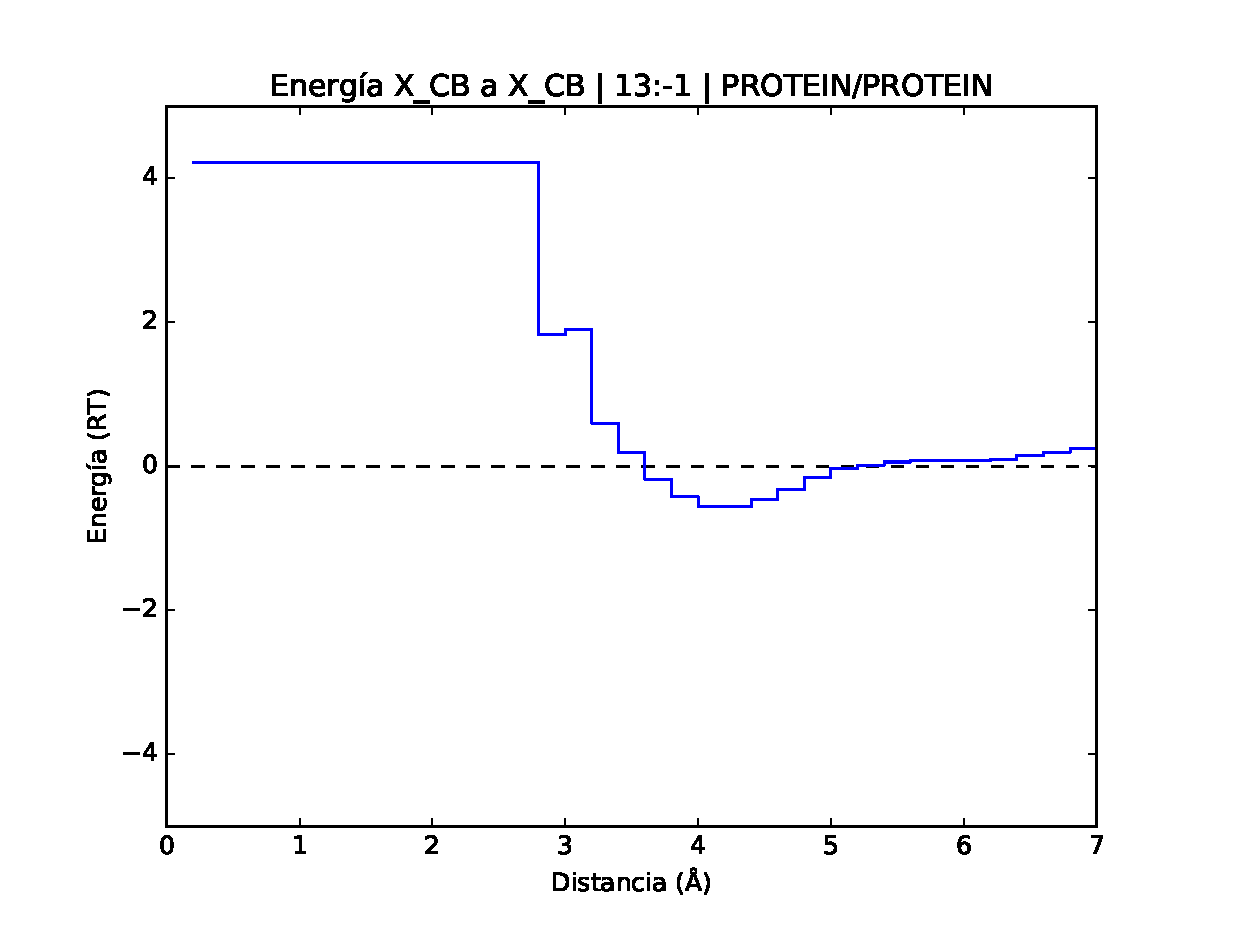
\includegraphics[width=\textwidth]{figures/prot_pot/eps_graphs/cb2cb.eps}
\caption{}
\end{subfigure}

\begin{subfigure}{.8\textwidth}
\centering
\includegraphics[width=\textwidth]{figures/prot_pot/eps_graphs/sh2sh.eps}
\caption{}
\end{subfigure}
\caption[Ejemplos de funciones de energía en proteínas]{Gráficos de las funciones de energía utilizadas en proteínas. 
En (a) se observa la energía (unidades RT) en función de la distancia en \si{\angstrom} para los carbonos beta de todos los aminoácidos. 
En (b) se tiene la función de energía para los átomos de azufre de císteina, representando los puentes disulfuro.}
\label{fig:energy1}
\end{figure}

\begin{figure}[p]
\includegraphics[width=\textwidth]{figures/prot_pot/mij.png}
\caption[Cálculo de $\sigma$]{Matriz de conteo de interacciones para los potenciales en proteína, o \textit{Mij}. 
Solo se usa el triángulo superior de esta estructura, ya que no se considera el orden de las interacciones. 
Conteos están en escala logarítmica para facilitar la visualización.}
\label{fig:mij}
\end{figure}
\cleardoublepage

\subsubsection{Derivación de potenciales basados en conteos de átomos}
\par
Estos potenciales están basados en el conteo de la cantidad de centros atómicos dentro de un rango de 7 \si{\angstrom} de un átomo.
Las frecuencias están basadas en \textit{bins} de 20 unidades con un máximo de 100 para todos los tipos de potenciales utilizados (ADN, ARN, proteínas).
Como no dependen de interacciones entre pares de átomos o distancias de residuos, se debe modificar la ecuación~\ref{ec:finalboltz}:

\begin{equation}
\Delta E^{i}(c) = RT\log \left[1 + M_{i}\sigma\right] - RT\log \left[ 1 + M_{i}\sigma \frac{f^{i}(c)}{f_{rel}} \right] \label{ec:surfboltz}
\end{equation}

Donde \textit{i} indica el tipo de átomo, \textit{Mi} es la cantidad de observaciones del átomo tipo \textit{i}, \textit{$f^{i}(c)$} es la frecuencia de observaciones en que un átomo \textit{i} tuvo \textit{c} átomos a su alrededor y \textit{$f_{rel}$} es la frecuencia esperada, equivalente a 1/(número de \textit{bins}).
El factor de corrección $\sigma$ se mantiene en 1/50.
Un ejemplo de funciones de energía puede ser visto en la figura~\ref{fig:inteng}, donde se muestra la energía en función de la cantidad de átomos alrededor para un carbono aromático y para un nitrógeno ácido.
La metodología de derivación tiene pequeños cambios aparte de utilizar la ecuación~\ref{ec:surfboltz}.
En el algoritmo~\ref{alg:intpot} se tienen los pasos para la derivación, donde podemos notar los cambios respecto al algoritmo~\ref{alg:deralgo1}.
\textit{Mij} pasa a ser \textit{Mi}, una lista con la cantidad de observaciones de cada tipo de átomo, \textit{Fij} pasa a ser \textit{Fi}, una única tabla con las frecuencias de cada átomo \textit{i} para cada \textit{bin} de conteo, y \textit{Fxx} pasa a ser un único valor, \textit{Frel}.

\begin{algorithm}[H]
\caption{Pasos para la derivación de un potencial de conteo a partir de una lista de archivos PDB}\label{alg:intpot}
\begin{algorithmic}[1]
\Procedure{GenerateCountPotential}{}
\State $ \text{matrix1D } Mi $ \Comment{Vector de conteo de átomos del tipo I en la base de datos}
\State $ \text{matrix2D } Fi $ \Comment{Tabla de frecuencias de conteo para cada tipo atómico y \textit{bin}}
\State $ \text{float } Frel $ \Comment{Frecuencia esperada, 1/\textit{bins} }
\State $ \text{list } pdblist \gets \text{GetPDBs}(argv1) $ \Comment{Carga estructuras PDB desde lista de archivos en disco}
\For {$ \textit{pdbstruct} \text{ in } \textit{PDBlist} $}
\State $ \text{CountEnv}(pdbstruct,Radius) $ \Comment{Calcula los átomos alrededor de otro átomo dentro del rango \textit{Radius}}
\EndFor
\State $ \text{CountCalculateIntFreq}(PDBlist,Fi,Frel,Mi,Nbins) $ \Comment{Calcula todas las tablas necesarias para la derivación del potencial}
\State $ \text{WritePotentialCount}(Fi,Frel,Mi,Nbins,Sigma) $ \Comment{Escribe el potencial creado a disco}
\EndProcedure
\end{algorithmic}
\end{algorithm}


\begin{figure}[p]
\centering
\begin{subfigure}{.8\textwidth}
\centering
\includegraphics[width=\textwidth]{figures/prot_pot/coarse/aromatic.eps}
\caption{}
\end{subfigure}

\begin{subfigure}{.8\textwidth}
\centering
\includegraphics[width=\textwidth]{figures/prot_pot/coarse/nh_acids.eps}
\caption{}
\end{subfigure}
\caption[Ejemplos de funciones de energía para conteo de átomos en proteínas]{En (a) se puede observar la energía en función del conteo de átomos en un rango de 7 \si{\angstrom} para carbonos aromáticos en proteínas. En (b) se puede observar otra función, pero para nitrógenos ácidos de los aminoacidos asparagina y glutamina.}
\label{fig:inteng}
\end{figure}
\cleardoublepage

\subsection{Cálculo de la superficie accesible al solvente de una molécula}
\par
Para el cálculo de la superficie accesible al solvente o SASA se utilizó el llamado algoritmo de Shrake y Rupley (\cite{Shrake1973}), descrito en el algoritmo~\ref{alg:shrkrply1}. Este consiste generar para cada átomo de una estructura una nube de puntos con forma esférica que están a una distancia de radio de Van der Waals más el radio de una molécula de una molécula de agua del centro del átomo. 
Cada punto representa un área equivalente al área de una esfera con el radio descrito anteriormente dividido por el número de puntos.
Al eliminar los puntos que se encuentran en el interior del volumen de las nubes de puntos de otros átomos, es posible obtener la superficie accesible al contar los puntos restantes y multiplicarlos por el valor de superficie que representan.
En la figura~\ref{fig:thomsonfig} se pueden observas las divisiones del área de una esfera que estos puntos representan.
\par
La nube de puntos debe tener todos sus puntos lo más equidistantes posible en el plano esférico para que el cálculo de superficie no tenga sesgos debido a la distribución desbalanceada de los puntos.
Esto se logró utilizando nubes de puntos precalculadas utilizando el por el software Thomson Applet (\cite{Saff1997,thomson}) de 15092 puntos. 

\begin{algorithm}[H]
\caption{Pasos para la obtención del SASA de una estructura }\label{alg:shrkrply1}
\begin{algorithmic}[1]
\Procedure{CalculateSASA}{}
\State $ \text{pdbstrudct } pdb $ \Comment{Estructura PDB}
\State $ \text{matrix2D } unitsphere $ \Comment{Matriz de 3xN con las coordenadas 3D de la nube de puntos en una esfera unitaria}
  \For {$ \textit{atomI} \text{ in } \textit{pdbstruct} $}
    \State $ \text{matrix2D } points \gets unitsphere * (atom.vdw + 1.4) + atom.coords $ \Comment{Escala y mueve una copia de la nube de N puntos a las coordenadas del átomo actual}
    \State $ \text{int } surfacepoints \gets N $ \Comment{Contador de puntos expuestos al solvente}
    \State $ \text{float } totalSASA \gets 0 $ \Comment{Superficie expuesta final}
    \For{$  \textit{atomJ} \text{ in } \textit{atomI.interactions}  $} \Comment{Itera sobre los átomos J que interactuan con I}
      \For{$  \textit{point} \text{ in } \textit{points}  $}
        \If {$\text{IsPointInVolume}(atomJ,point) \text{ and } point.enabled$} \Comment{Revisa si el punto esta adentro del volumen del átomo J y si no fue contado antes}
          \State $ surfacepoints -= 1  $ \Comment{Decrementa el contador de puntos}
          \State $ point.enabled = False $ \Comment{Desabilita el punto, ya que no es necesario volver a revisarlo}
        \EndIf
      \EndFor
    \EndFor
    \State $ atomI.SASA \gets surfacepoints * atomI.tAREA / N $ \Comment{Calcula área del átomo}
    \State $ totalSASA \gets atomI.SASA + totalSASA $ \Comment{Suma el área al área total}
  \EndFor
\State $ \Return \textit{ totalSASA } $ \Comment{Retorna el SASA final}

\EndProcedure
\end{algorithmic}
\end{algorithm}

\begin{figure}[p]
\centering
\centering
\includegraphics[width=\textwidth]{figures/thomson/thomson.png}
\caption[Esfera en el software Thomson Applet]{En este ejemplo podemos observar una esfera subdividida en 1000 áreas equivalentes. Inicialmente las subáreas son inicializadas con valores aleatorios, los cuáles son optimizados utilizando un algoritmo de relajación considerando cada punto como una carga eléctrica forzada a moverse sobre una esfera.}
\label{fig:thomsonfig}
\end{figure}
\cleardoublepage

\subsection{Cálculo de las subsuperfícies de interacción}
\par
Para calcular las subsuperfícies de interacción entre dos átomos, se debe extender el algoritmo~\ref{alg:shrkrply1}. Esto se hace re

\subsection{Derivación de potenciales basados en BSA}
\par
\subsection{Derivación de potenciales basados en SASA}
\par
\subsection{Cálculo del IP (\textit{Information Product})}

  %Resultados
  \newpage
\section*{RESULTADOS}
\addcontentsline{toc}{section}{RESULTADOS}
\par\refstepcounter{section}
\par


  %Discusion
  \cleardoublepage
\newpage
\section*{DISCUSIÓN}
\addcontentsline{toc}{section}{DISCUSIÓN}
\par\refstepcounter{section}
\subsection{Pruebas en proteínas}
\par
La primera prueba que se le hace a los nuevos potenciales BSASA y SASA es la clasificación de estructuras en nativas y no nativas, un problema considerado ya resuelto por una gran cantidad de software y métodos publicados. (citar metodos)
En la figura~\ref{fig:ferrada2009} podemos observar como los potenciales de la metodología nueva utilizando subsuperfices y la combinación con potenciales de superfície tienen peores resultados que los que utilizan distancias y la combinación de conteo de átomos y distancia.
Esto se debe al rango de interacción más corto que tienen los potenciales BSASA, que impide el reconocomiento de posibles interacciones no favorables más distantes (figura~\ref{fig:radii_int}) que no es capaz de observar ya que el rango máximo de distancia es equivalente a dos veces el radio de Van der Waals más 1.4 \si{\angstrom} de distancia, siendo 1.4 \si{\angstrom} el radio de una molécula de agua.
En la figura~\ref{fig:radii_int} podemos ver las distribuciones de la cantidad de interacciones entre pares de átomos para las estructuras utilizadas en la derivación de los potenciales en proteína.
\begin{figure}[!p]
\centering
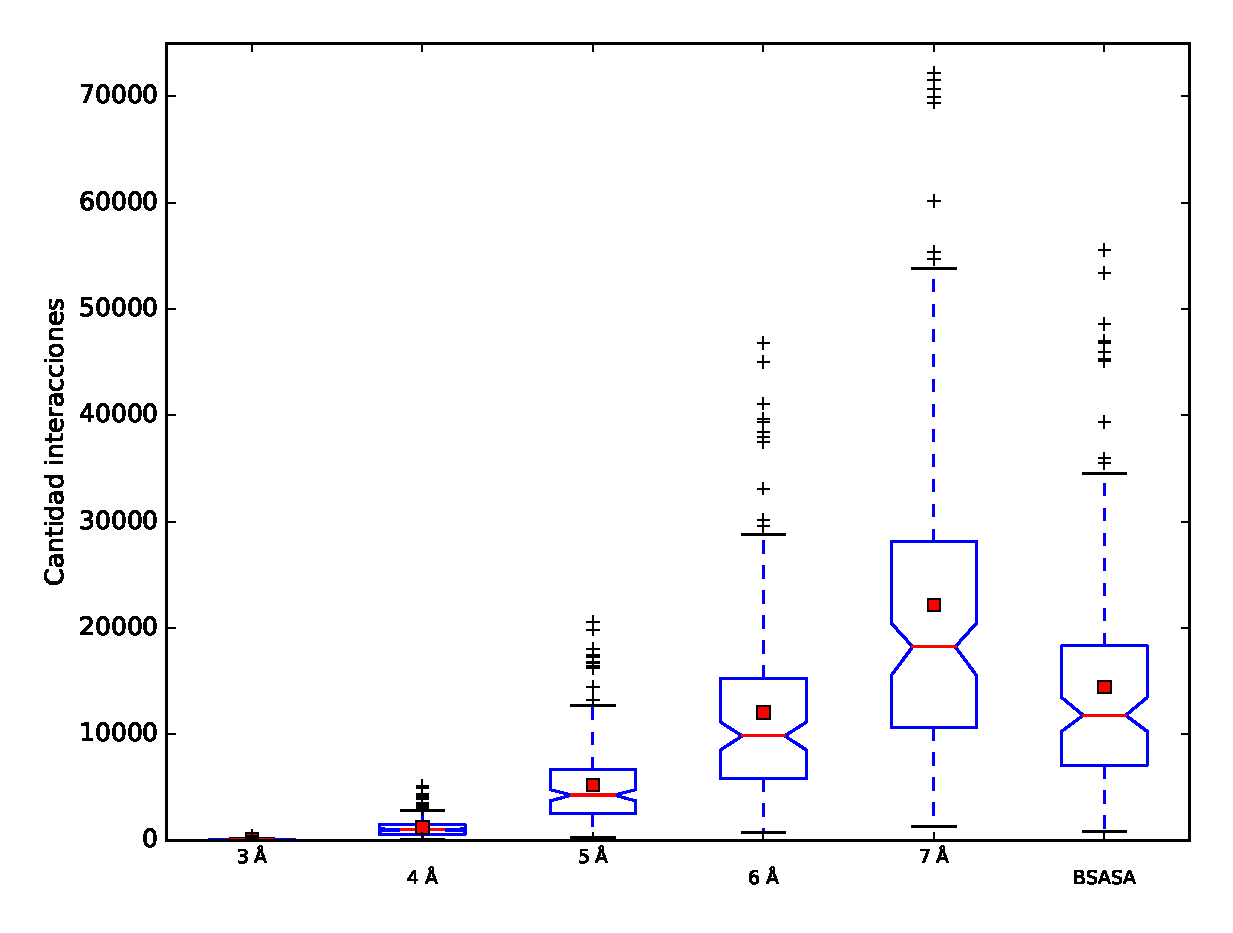
\includegraphics[width=\linewidth]{figures/radii_int.eps}
\caption[Boxplots de las distribuciones de la cantidad de contactos encontrados en el conjunto de estructuras usado en la derivación de potenciales para proteínas.]{Boxplots de las distribuciones de la cantidad de contactos encontrados en el conjunto de estructuras usado en la derivación de potenciales para proteínas. En la figura se tienen las distribuciones de la cantidad de contactos para potenciales dependientes de distancia variando el radio máximo de interacción de 3 a 7 \si{\angstrom}, más el potencial BSASA. La línea roja indica la mediana, el punto rojo el promedio, y la cintura el intervalo de confianza.}
\label{fig:radii_int}
\end{figure}
La distribución para BSASA muestra que el potencial evalua una menor cantidad de interacciones que los potenciales de distancia, que usan un rango de máximo de 7 \si{\angstrom} para evaluar interacciones.
De acuerdo a la ecuación~\ref{ec:ip} esto implica directamente que el potencial BSASA tiene un menor contenido de información disponible para la evaluación de la estructura, dado el menor número de interacciones pareadas observadas, que es el término \textit{n} en la ecuación.
Entre tanto, el potencial SASA logra un mucho mejor desempeño que conteo, dado que es mucho más fino en registrar si un átomo esta enterrado o expuesto, ya que se mide directamente la superficie en contacto con el solvente, en vez del método indirecto del potencial de conteo.
\par
En la segunda prueba, la capacidad de los nuevos potenciales BSASA y SASA en detectar errores aislados y expuestos en la superficie, tanto como errores más internos y difíciles de detectar fue evaluada utilizando perfiles de energía, en vez de usar el valor promedio de energía como en las pruebas anteriores.
Estos perfiles de energía contienen valores de energía promediados en una ventana deslizante de 7 residuos lo que permite eliminar variaciones bruscas en los valores de energía de cada residuo.
En esta prueba el valor final de energía de cada residuo se evalúa como un elemento independiente.
Al evaluar los errores de clase A, notamos que el desempeño de los pares de potenciales comparables no es distinguible, excepto en el caso de los potenciales SASA y CONTEO.
Dado que los errores en los residuos clase A son en residuos aislados y expuestos, el mejor desempeño de SASA versus CONTEO era esperado.
A su vez, los potenciales DD y BSASA y sus respectivas combinaciones DD+CONTEO y BSASA+SASA no muestran diferencias significativas en estos modelos.
Pero en los modelos clase B, cuyos residuos poseen errores más internos en la estructura afectando también residuos correctamente modelados su alrededor o entorno local, los potenciales BSASA y BSASA+SASA logran un desempeño superior a los potenciales DD y DD+CONTEO.
Esto se debe a la capacidad del potencial BSASA de excluir naturalmente los contactos que están escondidos detrás de otros átomos, algo que los potenciales de distancia no pueden detectar normalmente sin utilizar algoritmos para la detección de esos casos. (\cite{Ferrada2007,Ferrada2009})

\subsection{Pruebas en RNA}
En la primera prueba se observó la correlación del valor de energía calculado por los potenciales con las medidas de desviación estructural de más de 80 estructuras con 500 modelos cada una.
Esta prueba es muy similar a la primera prueba en proteínas, que buscaba separar modelos entre nativos y no nativos, que no es aún posible realizar dada la falta de una base de datos de estructuras y modelos de ARN ya clasificados en nativos y no nativos.
Al igual que en la primera prueba en proteínas, los potenciales BSASA y su combinación BSASA+SASA tienen un desempeño menor al potenciale de referencia RASP.
El potencial RASP utiliza un rango de 10 \si{\angstrom} para la detección de interacciones, lo que significa que es capaz de detectar y evaluar motifs de estructuras terciarias estadisticamente probables de estar en proximidad.
En la figura~\ref{fig:radii_rna}

  %Conclusiones
  \newpage
\section*{CONCLUSIONES}
\addcontentsline{toc}{section}{CONCLUSIONES}
\par\refstepcounter{section}
\par


  %bibliografia
  \newpage
\section*{REFERENCIAS}
\addcontentsline{toc}{section}{REFERENCIAS}
\begin{singlespace}
\printbibliography[heading=none]
\end{singlespace}

\end{document}
